\section{Data}
\label{sec:data}
This section explains the data. You may already know you could cite figures, see, e.g., Fig. \ref{fig:ng}.
\begin{figure}
    \centering
    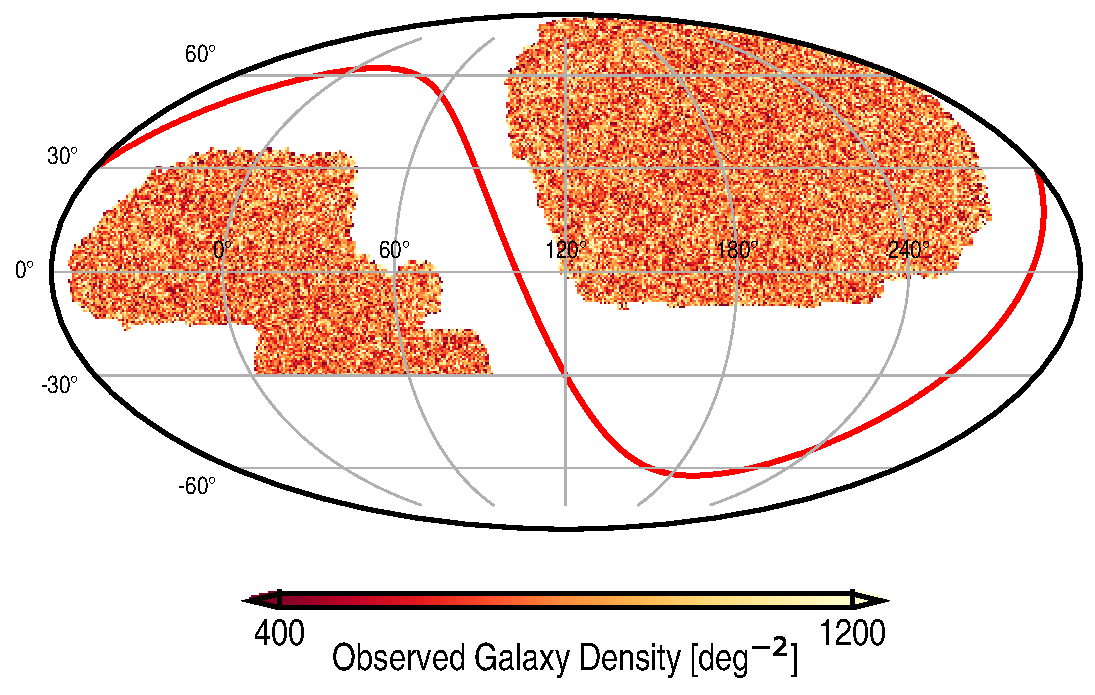
\includegraphics[width=0.45\textwidth]{figures/nlrg.pdf}
    \caption{Observed density field of DESI Luminous Red Galaxies DR9 in deg$^{-2}$}
    \label{fig:ng}
\end{figure}

And this is a table for you!
\begin{table}
  \begin{center}
    \caption{What about a table}
    \label{tab:ts}
    \begin{tabular}{lc}
    \hline
      \textbf{Criterion} &\textbf{Description}\\
      \hline   
     \textbf{DECaLS} & \\ 
     $z_{\rm fiber} < 21.7$  & faint limit  \\
     $z - W1 > 0.8 \times (r - z) - 0.6$ & Stellar rejection  \\
     $[(g-r >1.3)$ & Remove low-z galaxies \\
     $[(r-W1 > (W1 - 17.26)*1.8)$ & Luminosity cut \\ 
    \hline
     \textbf{BASS+MzLS} & \\ 
     $z_{\rm fiber} < 21.71$  & faint limit  \\
     $z - W1 > 0.8 \times (r - z) - 0.6$ & Stellar rejection  \\
     $[(g-r >1.34)$ & Remove low-z galaxies \\
     $[(r-W1 > (W1 - 17.24)*1.83)$ & Luminosity cut \\ 
      \hline
      \end{tabular}
  \end{center}
\end{table}